\documentclass{article}

\usepackage{graphicx}
\usepackage{amsmath}
\graphicspath{ {images/} }
\usepackage{amssymb}
\usepackage[left=3cm,top=2cm,right=3cm,nohead,nofoot]{geometry}
\usepackage{latexsym}
\usepackage{epsfig}
\parindent0pt
\parskip6pt
\pagestyle{empty}
%\pagestyle{empty}
%\usepackage{fancybox}
\usepackage{pstcol}
\newcommand{\R}{{\mathbb R}}
\title{MATH 444 Problem Set 2}
\author{Connor Wolfe}
\begin{document}
\maketitle

\section*{Problem 1}

\subsection*{Part (a): Designing the Algorithms}

\subsubsection*{Overview}

The first problem asks us to analyze the iris data set using the k-means and k-medoids algorithms.  The iris data set is a matrix corresponding to flower characteristics for three types of flowers: iris setosa, iris versacolor, and iris virginica.  This data set is a useful learning tool for clustering algorithms because there is a clear cluster between setosa and versacolor/virginica, but a more subtle cluster between versacolor and virginica.  The algorithm relies on the data file 'IrisDataAnnotated.mat' which contains two matrices: 
\begin{verbatim}  Data set X which contains the sepal length, sepal width, petal length, and petal 
  width of 150 sample flowers 
  
  Annotation vector I indicates Iris species such that:
        1= Iris setosa
        2=Iris versacolor
        3=Iris virginica
\end{verbatim} 

Part (a) of this problem asks the student to write a k-means and k-medoids algorithm.  I will outline both below:

\subsubsection*{K-means algorithm}
My k-means algorithm follows the template from lecture of: Fix parameters, Randomize initial partitioning, Iterate (update cluster centroids + re-assign points to clusters) and Analyze tolerance.  The following is a more in-depth analysis of the code:

\begin{itemize}
    \item \textbf{Fix Parameters} (lines 4-7) \\
    set k=3 (number of clusters) \\
    t=0.001 (want change in tightness to be less than t in order to break iteration.  Value chosen based on trial and error)
    dq=10 (initialize dq>t so that enter while loop on initialization) \\
    old\_q is just initialized to 0 to ensure we enter the while loop  \\
    time=0 (increment after each run of while loop)
    
    \item \textbf{Initialize} (lines 11-15)\\
    I used a random initialization to ensure correctness of algorithm \\
    First I define a vector 'A' as a random ordering of the numbers 1:150 (length of X matrix). I will use this random ordering of indices to set the initial clusters \\
    Then I define two randomly generated numbers, r1 and r2, to be between 40 and 60.  These variables will determine the lengths of the initial clusters so I restricted their range so that the clusters would have roughly equal sizes (~50)\\
    I then set the first cluster, I\_1 as the first 'r1' elements of A, the second cluster I\_2 as the next 'r2' elements of A, and the remaining elements in I\_3
    Note that the clusters I\_1,I\_2, and I\_3 do not have data for the elements within them, only indices to their location in X
    
    \item \textbf{Iteration:} (lines 31-45)\\
    \begin{itemize}
        \item \textbf{Update} (lines 31-33)\\
        I calculate the centroid of each cluster c1,c2, and c3 by summing the data of each dimension in the cluster divided by the cardinality of the cluster.  The Matlab code to do so looks like:\\
        31: c1=sum(X(:,I\_1),2)/size(I\_1,2); \\
        which equivalently yields:\\
        \[c1=\frac{1}{D_1} \sum_{j\epsilon I\_1} X^{(j)}\]
        We can see that we sum each dimension of elements in X that belong to I\_1 and divide each dimension by the length of vector I\_1
        \item \textbf{Assignment} (lines 35-45)
        First we iterate through the points in X and calculate their distance to each centroid as follows (using c1 as an example):\\
        \begin{verbatim}37: sqrt(sum((X(:,ind)-c1).^2));\end{verbatim}\\
        We store these values in a 3x150 dist matrix (3 corresponds to distance to each centroid, and 150 corresponds to each data point in X)\\
        Next we minimize the dist matrix about each 150 columns as such:\\
        \begin{verbatim}39: [m,i] = min(dist)\end{verbatim}\\
        where m is a 1x150 matrix corresponding to the distance of each X to its closest centroid and i is a 1x150 matrix corresponding to which centroid (1, 2, or 3) that distance is relative to\\
        Finally, we can reassign clusters I\_1, I\_2, and I\_3 by assigning the indices within the i matrix to their corresponding cluster.  For example, for cluster 1 we write:\\
        \begin{verbatim}43: I_1=find(i==1);\end{verbatim}
    \end{itemize}
    
    \item \textbf{Analyze} (lines 47-49)\\
    Finally, we recompute q easily as the sum of the values in m, the minimum distance matrix.  We calculate dq as the difference between  new\_q and old\_q and reset old\_q as the current new\_q to prepare for the next iteration.  This ends the while loop and we will check the condition if dq is less than the tolerance defined in step 1
    
\end{itemize}

\subsubsection*{K-medoids algorithm}
My K-Medoids follows a similar template of: Fix parameters, Randomize 3 initial medoids, Iterate (assign to closest medoid + update cluster medoid) and Analyze tolerance.  The following is a more in-depth analysis of the code:

\begin{itemize}
    \item \textbf{Fix Parameters} (lines 4-15) \\
    set k=3 (number of clusters) \\
    t=0.001 (want change in tightness to be less than t in order to break iteration.  Value chosen based on trial and error)
    dq=10 (initialize dq>t so that enter while loop on initialization) \\
    old\_q is just initialized to 0 to ensure we enter the while loop \\
    time=0 (increment after each run of while loop)\\
    Most importantly, I define a dist (150x150) matrix and fill it with the distance from each point to every other in X.  This will be useful because we will not need to recalculate this distance every time we compute a new medoid.  Note that in the k-medoids algorithm I will use l\_1 distance measure as follows: 
    \[||x-y||_1 = \sum_{j=1}^{n} |x-y|\] 
    
    \item \textbf{Initialize} (lines 18-20)\\
    I used a random initialization to ensure correctness of algorithm \\
    First I define a vector 'A' as a random ordering of the numbers 1:150 (length of X matrix). I then draw the first three randomly ordered elements of A and use them as the indices of the initial medoids.\\
    I store the medoids in matrix m (4x3) corresponding to the 4 fields of data for the 3 medoids.  I also store the indices of the medoids in vector m\_ind (1x3)
    
    \item \textbf{Iteration:} (lines 26-57)\\
    \begin{itemize}
        \item \textbf{Assignment} (lines 36-32)\\
        First I define matrix dist\_to\_all\_meds (150x3) as the distance of each medoid to all X values.  I do this by extracting the column corresponding to each medoid (referencing the medoid by using the m\_ind vector) from the dist matrix as follows:\\
            \begin{verbatim}26: dist_to_all_meds=[dist(:,m_ind(1)) dist(:,m_ind(2)) dist(:,m_ind(3))];\end{verbatim}\\
        by using the Matlab min function on dist\_to\_all\_meds, I define dist\_to\_closest\_med (1x150) which is the distance of each X to its closest medoid and cluster\_num (1x150) which is the cluster X is closest to (1, 2, or 3).
        Finally, as in K-Means, we can reassign clusters I\_1, I\_2, and I\_3 by assigning each index within the cluster\_num matrix to its appropriate cluster.  For example, for cluster 1 we write:\\
        \begin{verbatim}43: I_1=find(cluster\_num==1);\end{verbatim}
        
      
        \item \textbf{Update} (lines 44-62)
        In this step, we must find the best medoid for each cluster.  To do so we first create a new matrix c\_i which corresponds to the distances between only the elements within cluster i (extracted from the distance matrix.  For example, for cluster 1, we define c1 as follows:\\
        \begin{verbatim}c1=sum(dist(I_1,I_1));\end{verbatim}\\
        Next, we minimize c\_i to find the point which has the smallest sum of distances to the other points\\
        Last, update the m matrix and the m\_ind matrix to reflect this new medoid
       
    \end{itemize}
    
    \item \textbf{Analyze} (lines 47-49)\\
    Finally, we recompute q easily as the sum of the q from each cluster.  We calculate dq as the difference between  new\_q and old\_q and reset old\_q as the current new\_q to prepare for the next iteration.  This ends the while loop and we will check the condition if dq is less than the tolerance defined in step 1
    
\end{itemize}

\subsection*{Part (b): Analysis of the Algorithms}
    In the second part of problem 1, we are asked to run the k-means and k-medoids algorithms with a random initialization.  
   \subsubsection*{K-Means}
    First I will show the graphs for each iteration of one well-clustered run of k-means in figure (1). We can see the random initial clustering is drastically changed by iteration two, when setosa has essentially been properly classified.  The remaining iterations attempt to distinguish between versacolor and virginica with a success rate I will explore next.
    \begin{figure}[h!]
    \centerline
    {
    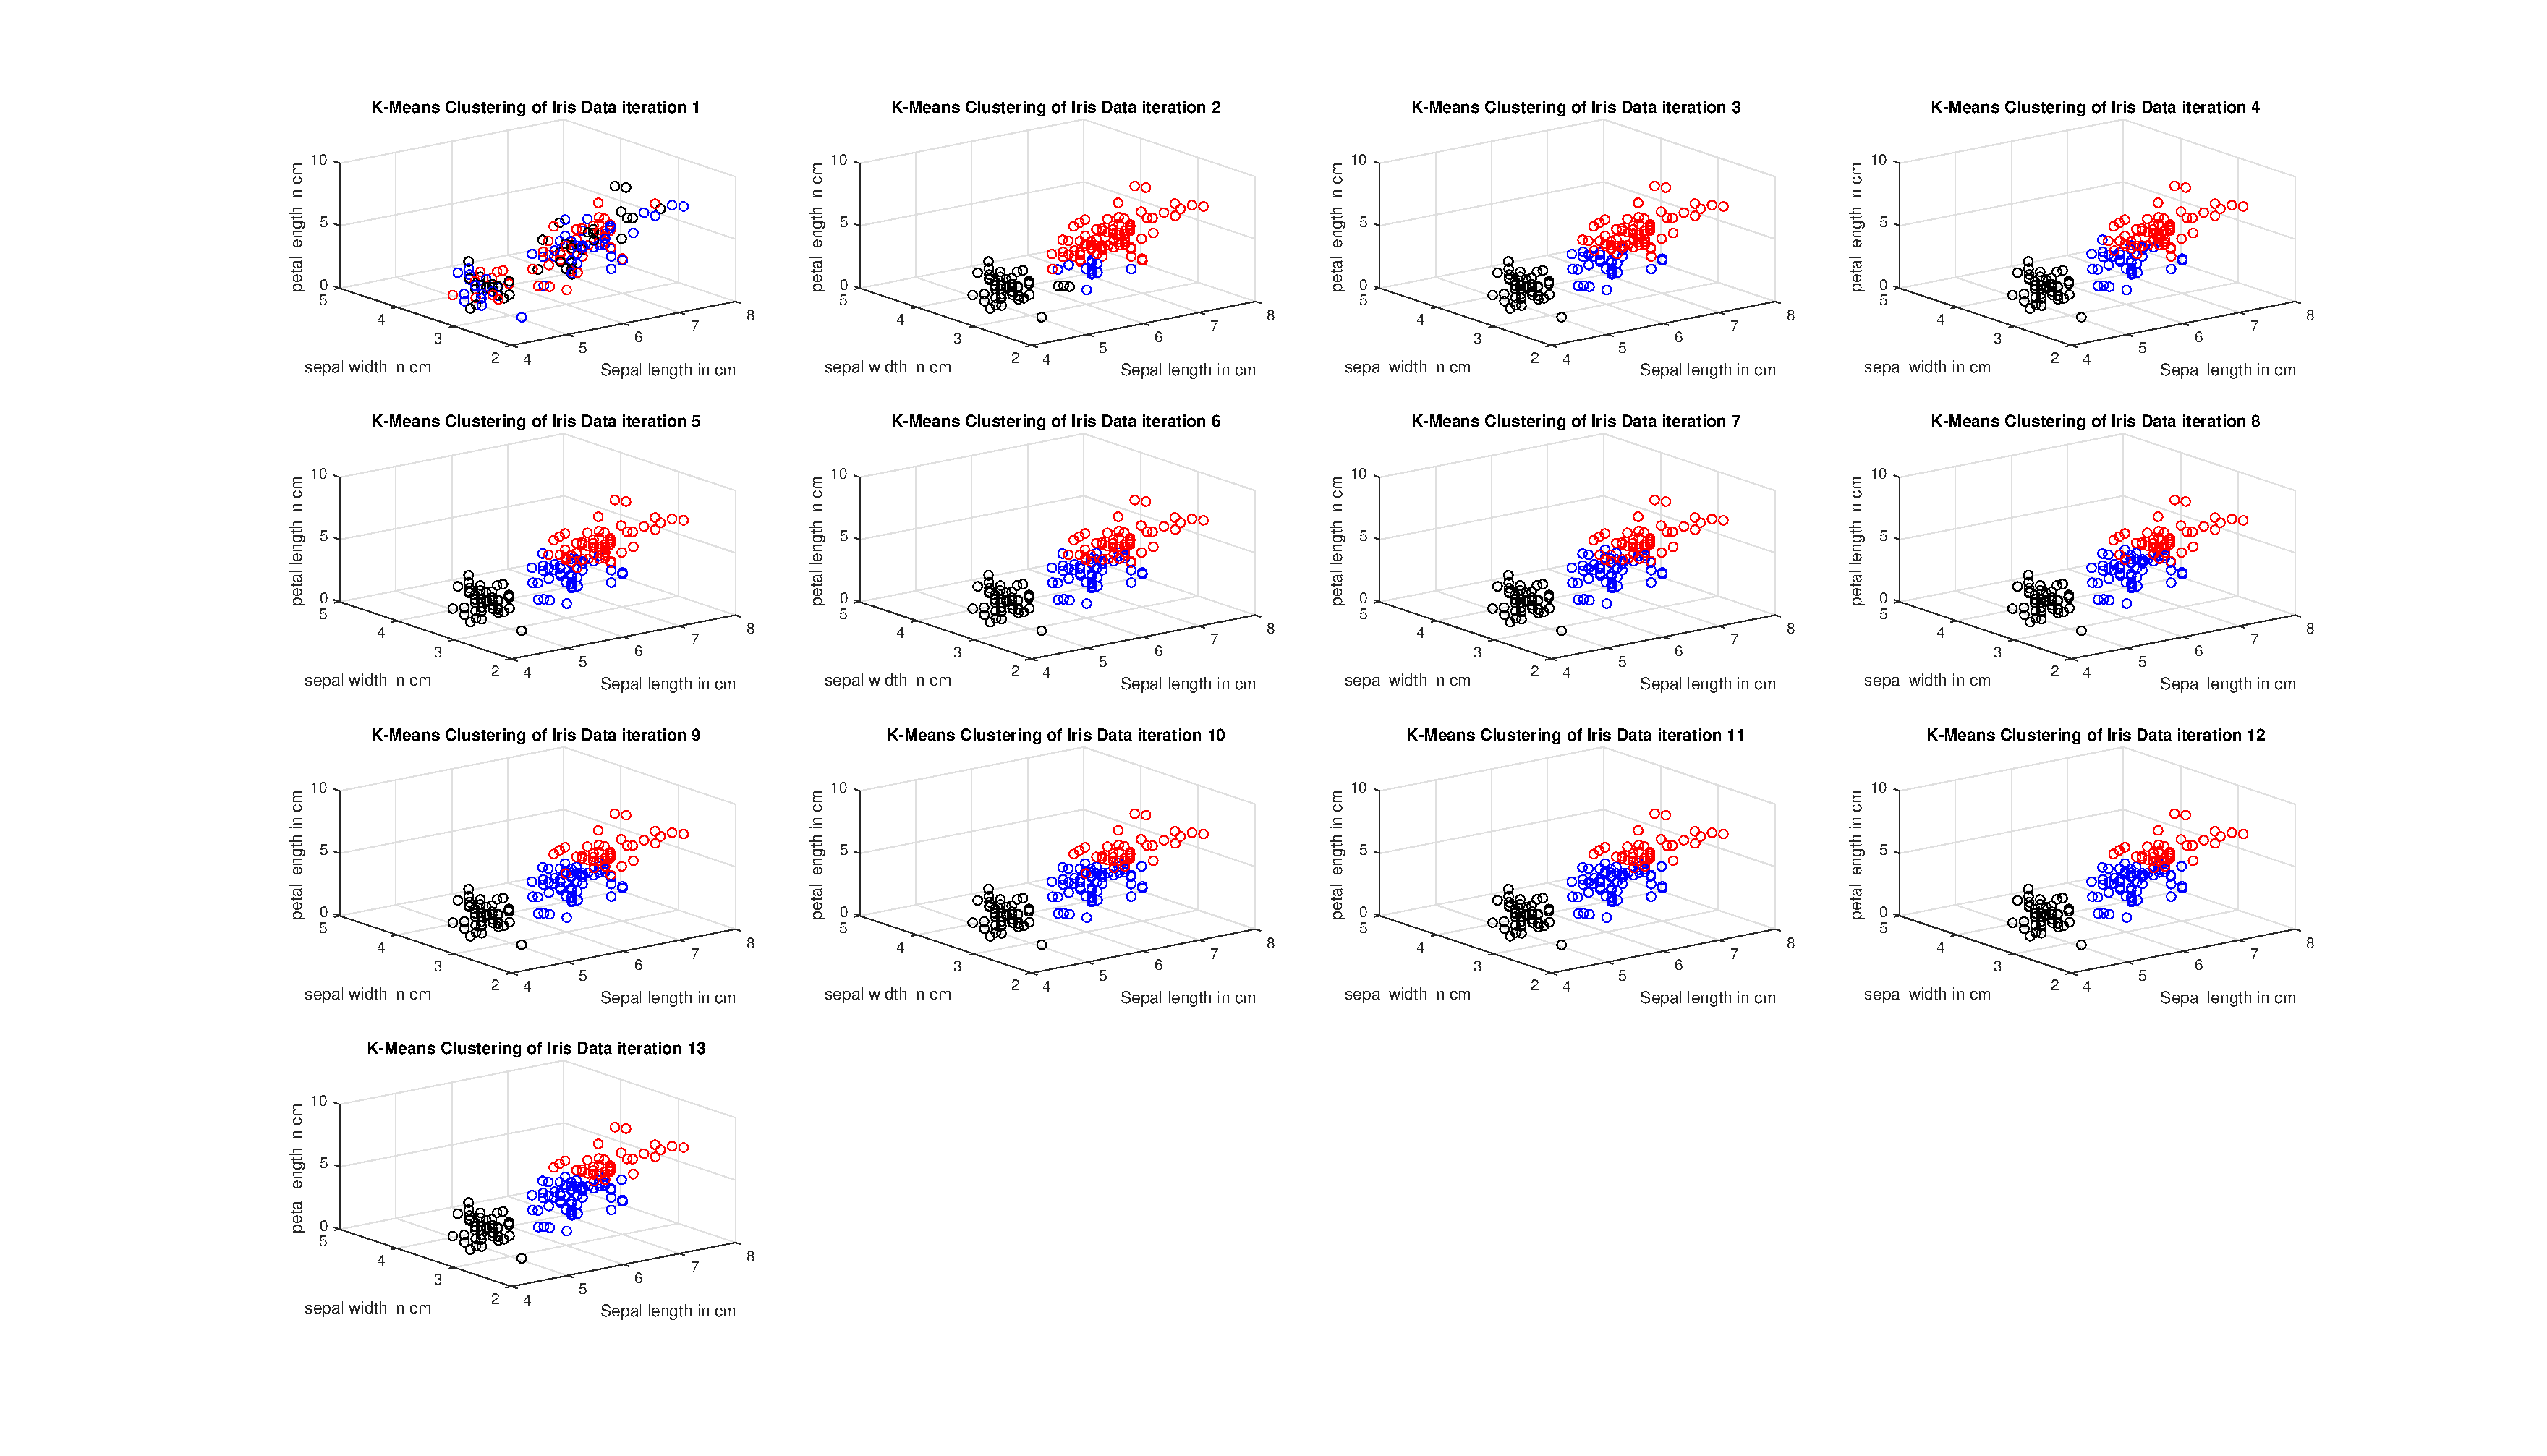
\includegraphics[width=20cm, height=10cm]{kmeans_iterations}\\
    }
    \caption{\label{fig:my figure} plot of each successive iteration of k-means on the iris data set.  As the iteration number increases we can clearly see the data become more clustered}
    \end{figure}

    Next I analyzed the robustness of the algorithm over repeated trials.  Figure (2) shows a table representing the number of misclassifications per 10 trials.  I calculated these values with the following methodology.  I defined a 3x3 matrix 'class' to store the number of each flower type that each cluster classified.  I then iterated over the three clusters I found and incremented the appropriate column for each type of flower the cluster held.  I then took the max of the class vector, which yields a 1x3 vector with the numbers 1, 2, and 3 ordered somehow.  The location of the 1 within this vector is the index of the cluster representing setosa, and 2 for verrsacolor/3 for virginica.  For instance, if 1 is the second element of the vector, then that means that I\_2 corresponds to setosa.  The class matrix contains how many of each flower type the cluster holds, so now that we know which cluster is which flower, we can add up the misclassifications.  The table in the left panel of figure 2 shows the results of such an analysis for 10 trials.\\
    
    This analysis of k-means demonstrates that it is very effective at distinguishing between setosa and versacolor/virginica (90 \% success), but distinguishing between versacolor and virginica is challenging for kmeans (consistently misclassifying 17/100 of these flowers).  The data for these two flowers is not ideal for clustering as there is no clear dividing point between the two in the graph, and therefore clustering by a distance measure will never prove effective on these flowers as the data from one can be identical to the data from another.  
    
    \begin{figure}[h!]
    \centerline
    {
    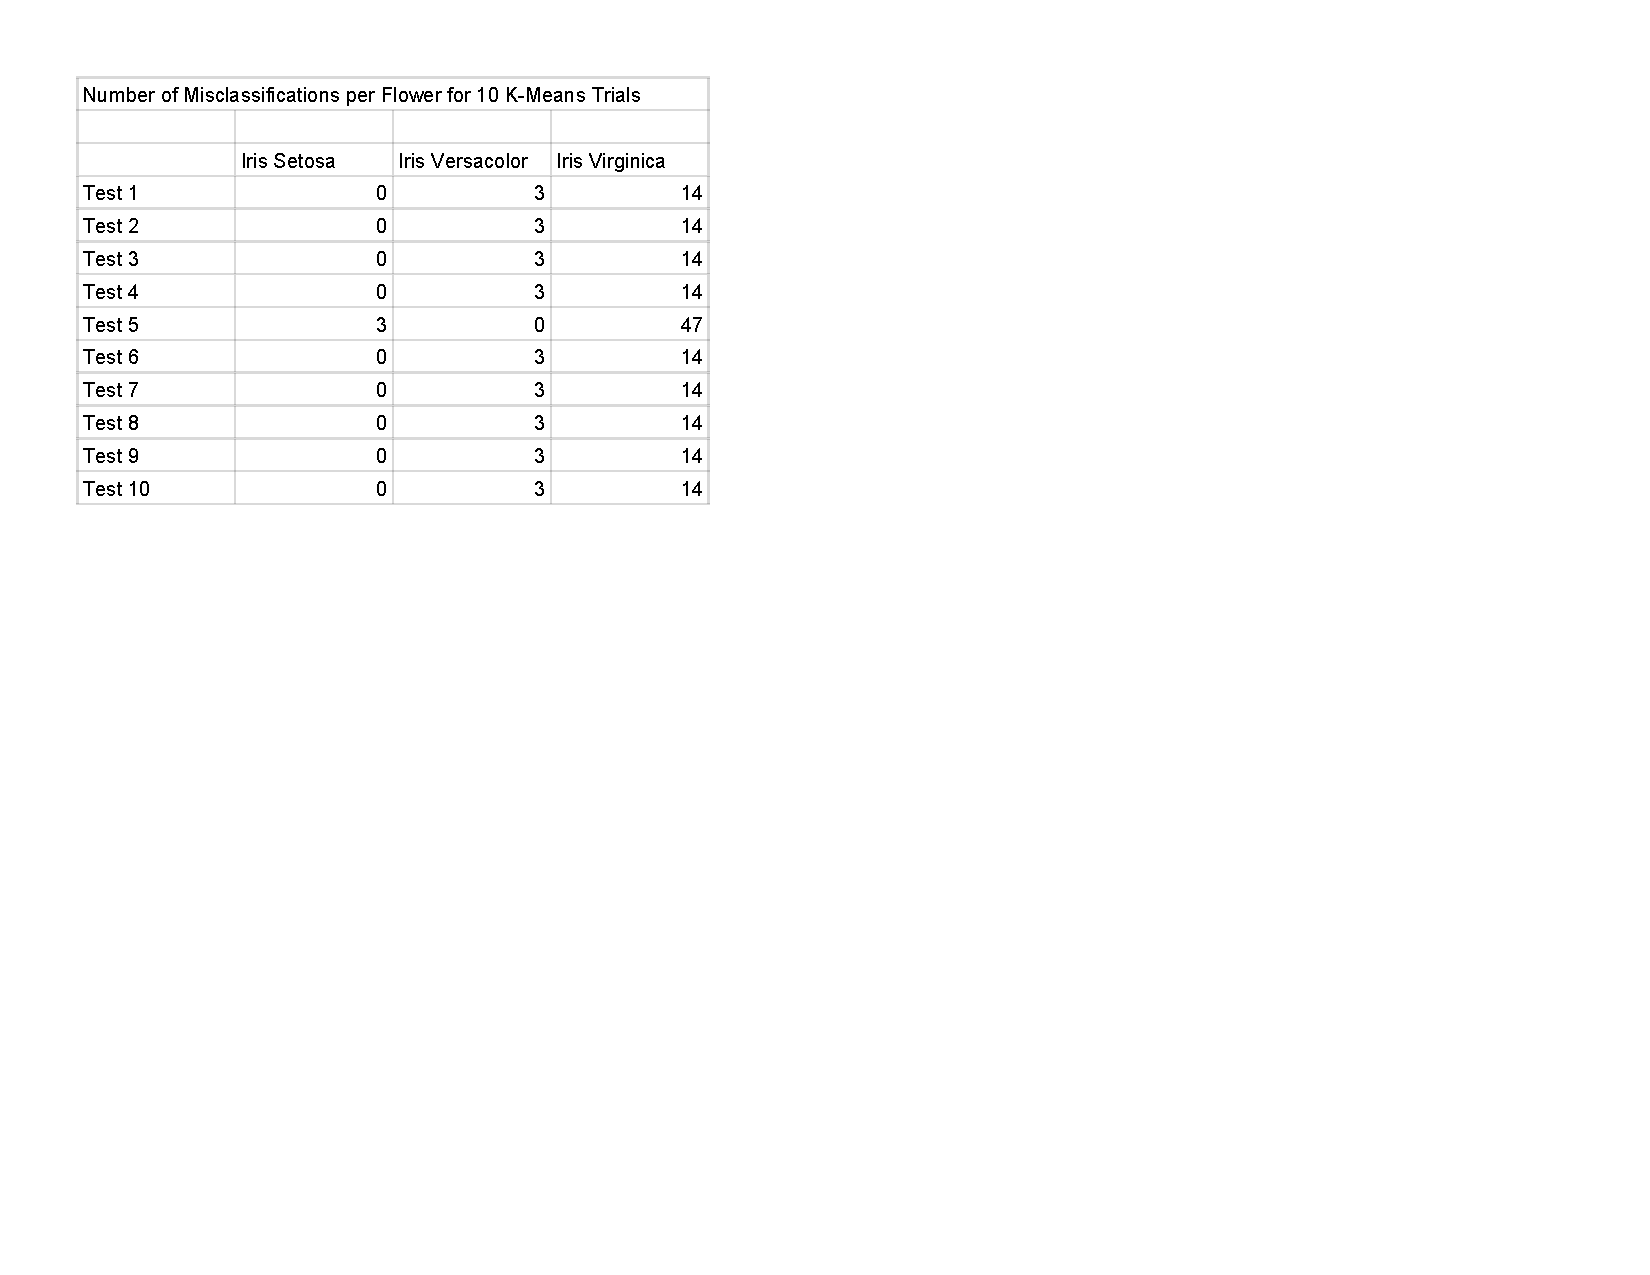
\includegraphics[width=10cm, height=5cm] {num_miscl_kmeans} 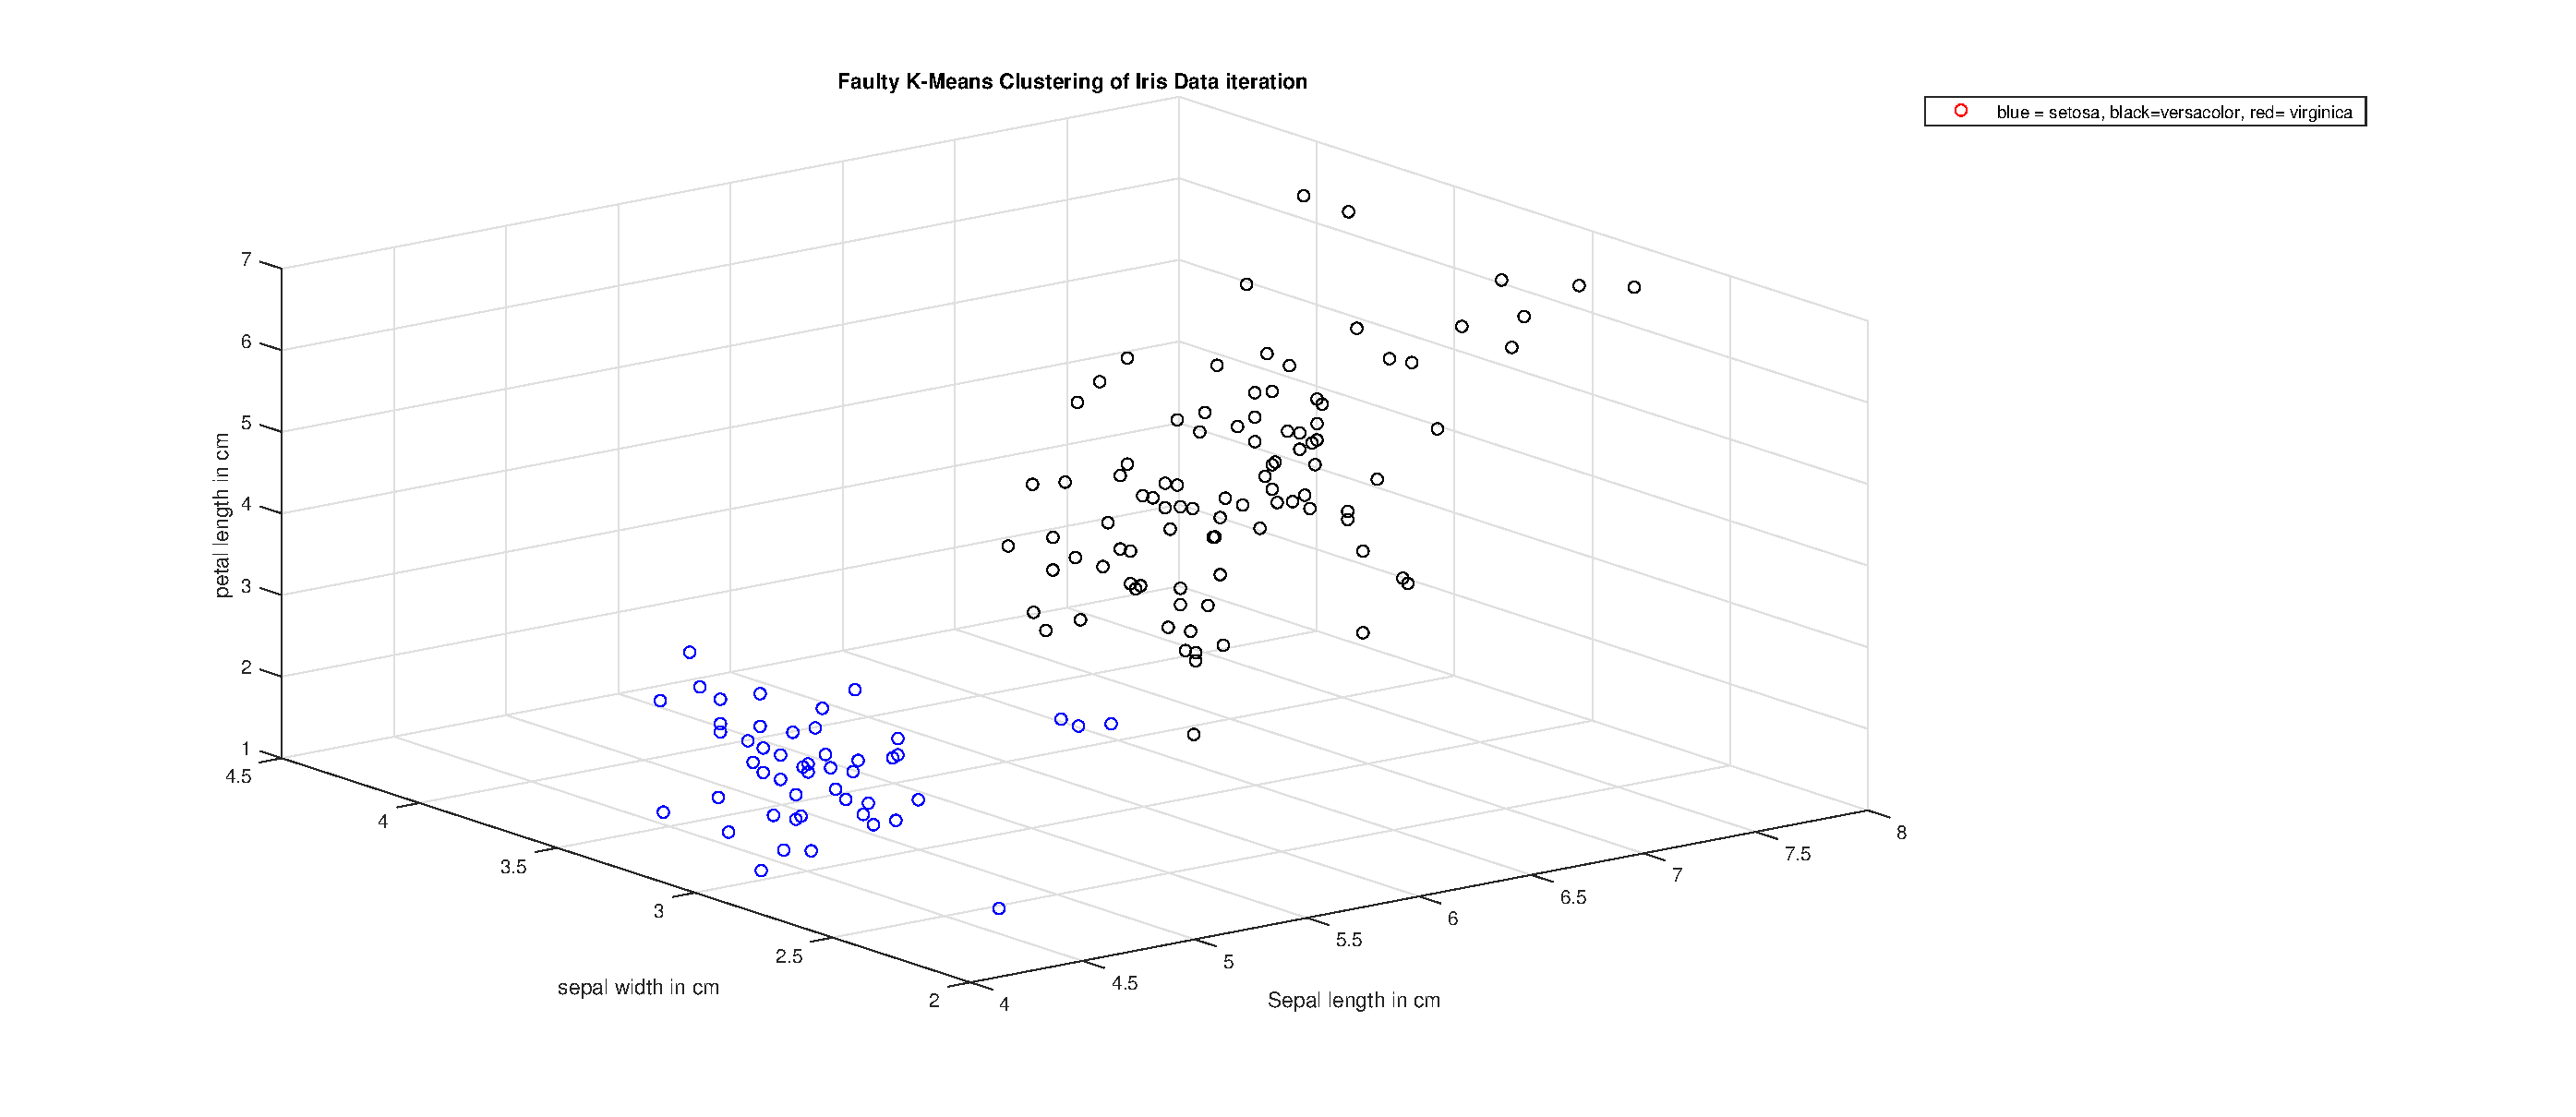
\includegraphics[width=10cm, height=5cm]{bad_k_means_cluster}
    }
    \caption{\label{fig:my figure} The number of misclassifications 10 trials of k-means made per flower type.  We can see that the algorithm successfully clusters 9/10 trials, except on trial 5 when it clusters virginica and versacolor together.  The right panel shows the graph of this misclustering }
    \end{figure}
    
    \subsubsection*{K-Medoids}
    Again, I begin by showing the graphs for every iteraton of a succesful run of k-medoids in figure (3).  We can see the random initial clustering is drastically changed by iteraton two, when setosa has essentially been properly classified.  The remaining iterations attempt to distinguish between versacolor and virginica with a success rate I will explore next.  \\
    \begin{figure}[h!]
    \centerline
    {
    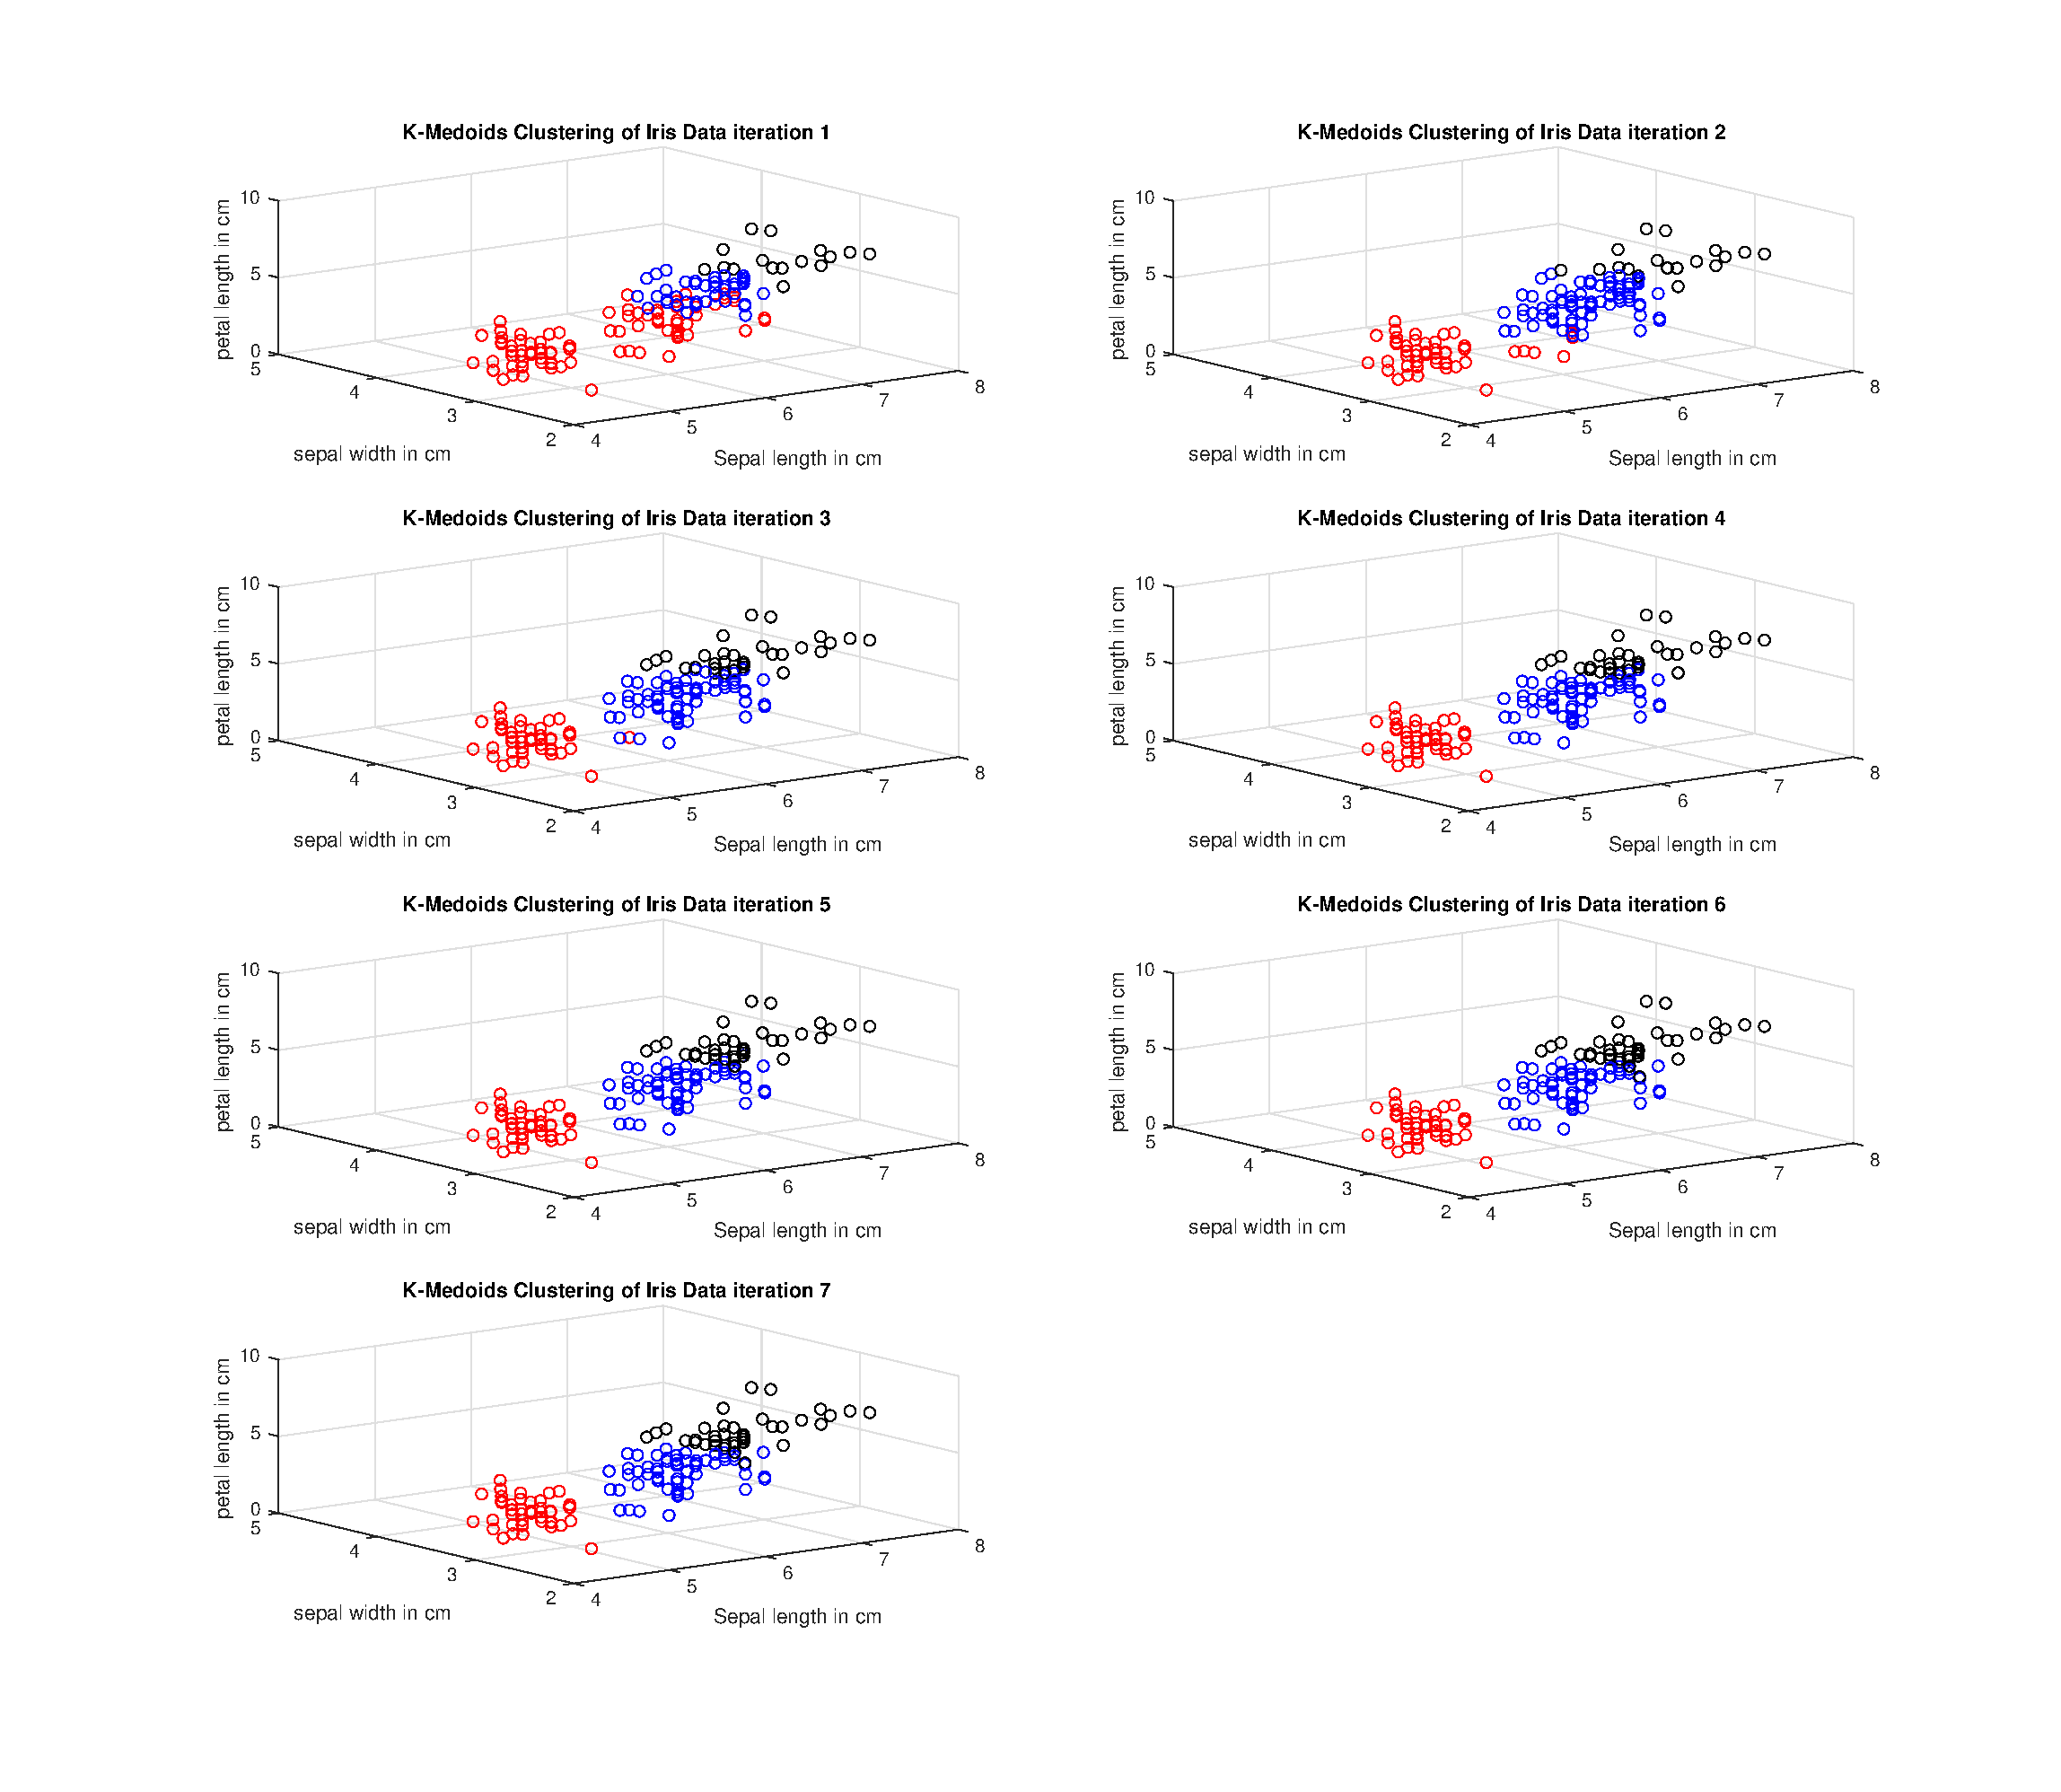
\includegraphics[width=15cm, height=7cm] {kmedoids_iterations}
    }
    \caption{\label{fig:my figure} plot of each successive iteration of k-means on the iris data set.  As the iteration number increases we can clearly see the data become more clustered }
    \end{figure}
    
    
    In order to analyze the robustness of k-medoids I applied the same methodology and code as for k-means.  Figure (4) shows the results of the 10 trials, calculated just as in k-means.  \\
    
    
    \begin{figure}[h!]
    \centerline
    {
    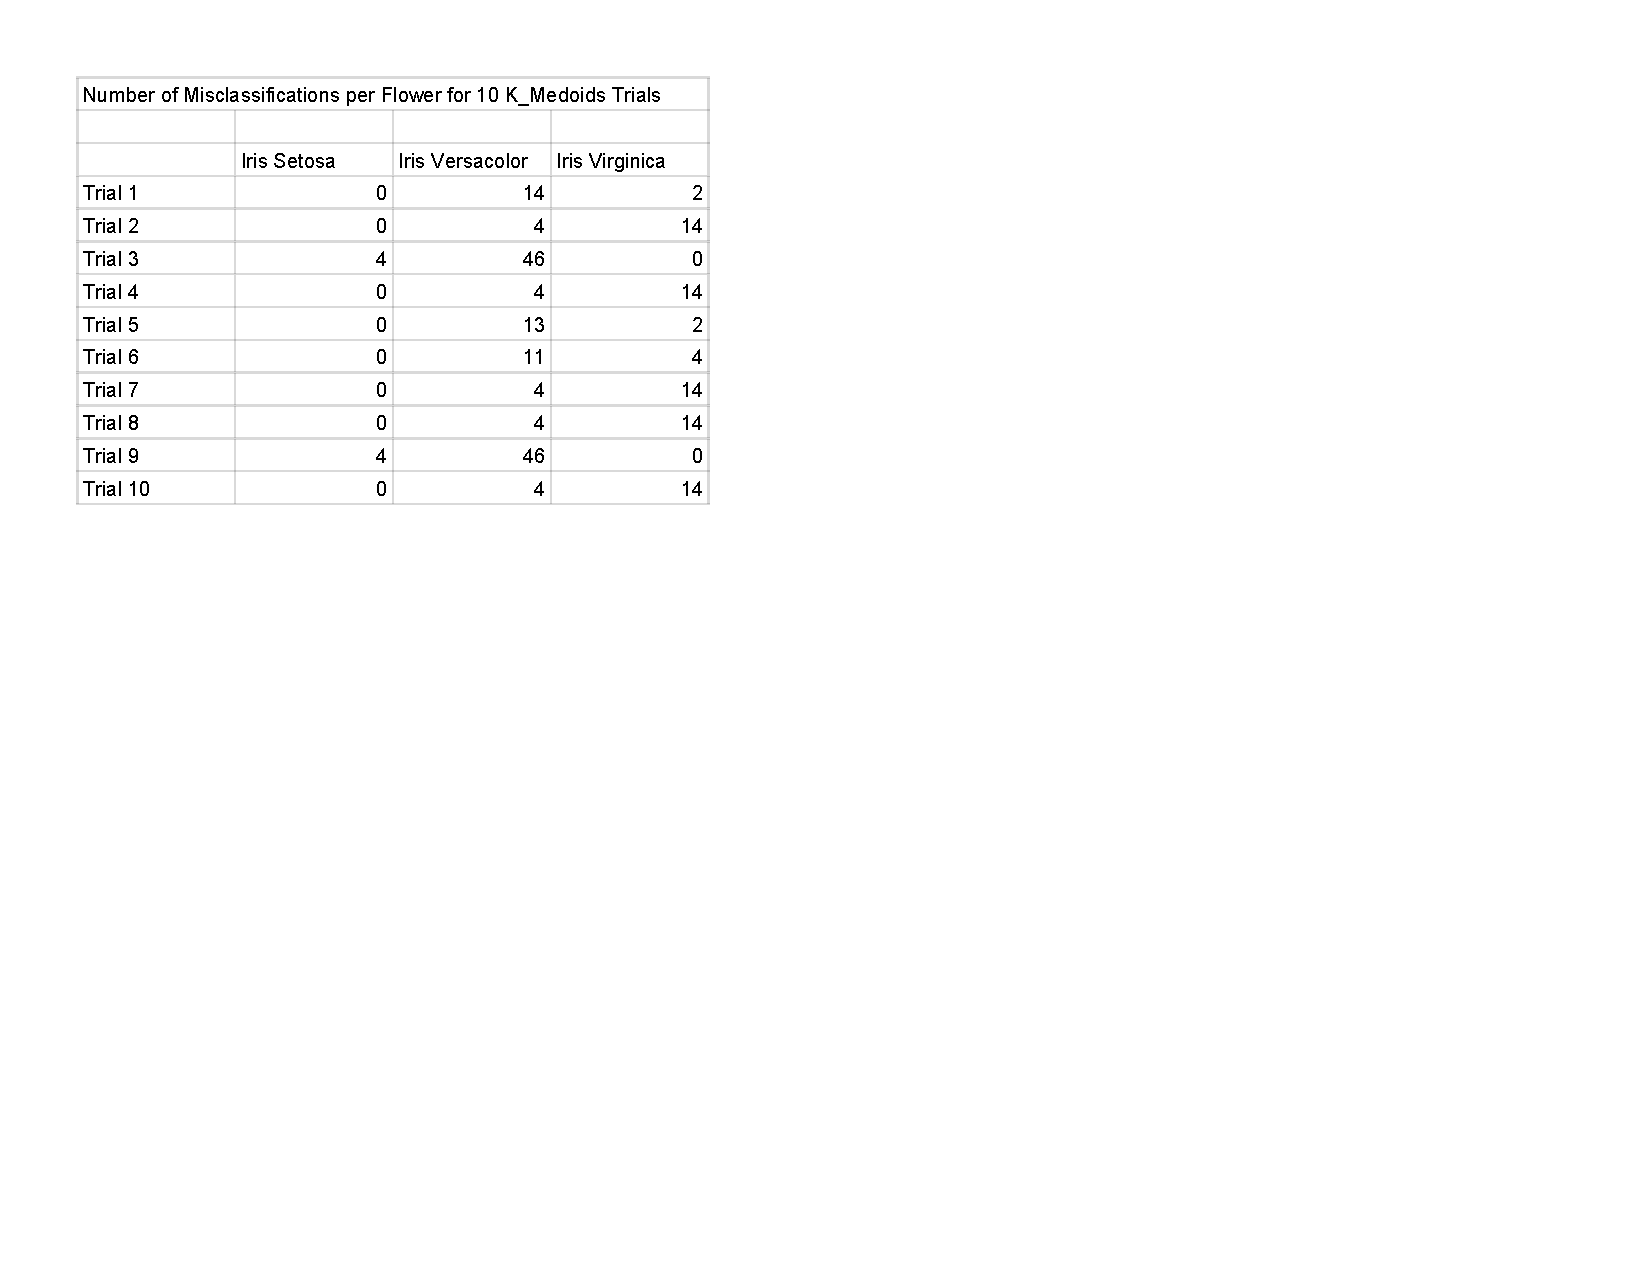
\includegraphics[width=8cm, height=4cm] {num_miscl_kmedoids} 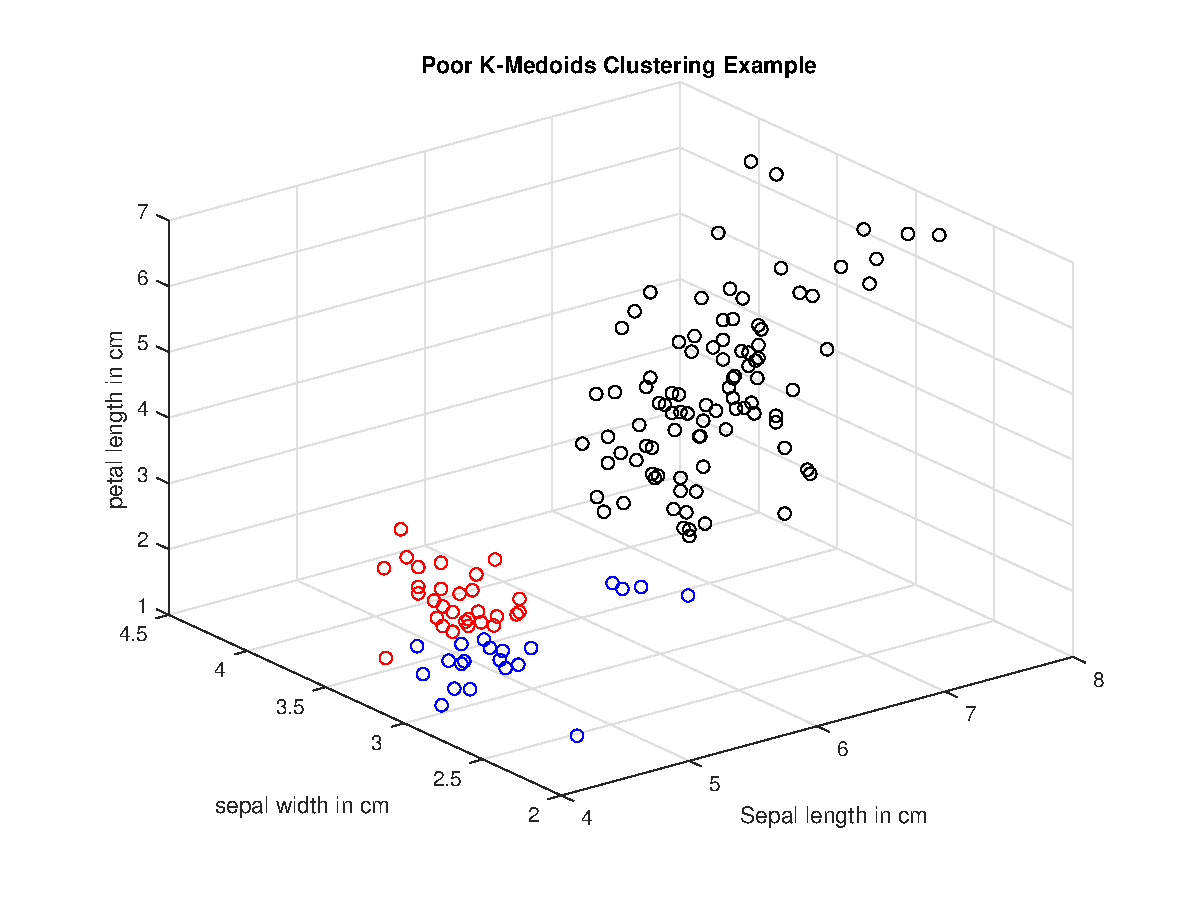
\includegraphics[width=8cm, height=4cm]{bad_k_medoids_cluster}
    }
    \caption{\label{fig:my figure} The number of misclassifications for 10 trials of k-medoids made per flower type.  We can see that the algorithm successfully clusters 8/10 trials. On trials 3 and 9, though, it clusters virginica and versacolor together.  The right panel shows a graph of this misclustering }
    \end{figure}
    
    This analysis of k-medoids demonstrates that it is very effective at distinguishing between setosa and versacolor/virginica (80 \% success), but distinguishing between versacolor and virginica is also challenging for kmeans (consistently misclassifying ~16/100 of these flowers).  The data for these two flowers is not ideal for clustering as there is no clear dividing point between the two in the graph, and therefore clustering by a distance measure will never prove effective on these flowers as the data from one can be identical to the data from another.
    
    
\bigskip


\section*{Problem 2}

\subsection*{Overview}
The second problem analyzes the data within 'BiopsyDataAnnotated.mat.'  This file contains a maxtrix X (6x999) which contains 9-dimensional biopsy data from 699 biopsies.  The data takes on values from 1-10.  The file also includes an annotation vector I, which classifies each biopsy in X as a benign (0) or malignant (1) tumor.  This problem asks us to run the k-medoids algorithm described above, using k=2 clusters.  After running k-medoids, we analyze the success of the clusters by calculating the rates of misclassification on repeated trials.  I used the same theory to as in problem 1 to identify which clusters stored which data.  I created a 2x2 class matrix, which corresponds to the number of points classified as benign/malignant for each cluster.  I then ran the 'max' function on this matrix, to yield which row in class corresponds to which cluster.  Using this information, I create two 1x2 vectors class\_benign and class\_malignant which hold the number of actually benign and actually malignant sample points each cluster holds.  The code for this is below:\\
\begin{verbatim}class_benign=class(find(b==1),:);
class_malignant=class(find(b==2),:);\end{verbatim}

Every trial that I run will produce the same medoids at index 435 and 23, which produces identical clustering.  Therefore my class\_malignant and class\_benign vectors had the same numbers each time.  class\_malignant=[9,216] and class\_benign=[435, 23].  This means that the code correctly clustered 216 of the malignant cases and 435 of the benign cases, but incorrectly clustered 9 malignant and 23 benign.

\subsection*{Sensitivity}
The sensitivity is mathematically defined as:
\[
\text{sensitivity} = \frac{\text{\# of malignant cases classified correctly}}{\text{ \# of all malignant}}
\]
I calculate the sensitivity by using the second dimension of the class\_malignant vector (the number of true malignant sample points are in this cluster) and divide it by the total number of malignant samples as follows:
\begin{verbatim}
sensitivity=class_malignant(2)/num_malignant;
\end{verbatim}

Given the repetition of my data, the calculation simplifies to sensitivity = 216/239 = 0.9038

\subsection*{Specificity}
The specificity is mathematically defined as:
\[
\text{specificity} = \frac{\text{\# of benign cases classified correctly}}{\text{ \# of all benign}}
\]
I calculate the specificity by using the first dimension of the class\_benign vector (the number of true benign sample points are in this cluster) and divide it by the total number of benign samples as follows:
\begin{verbatim}
specificity=class_benign(1)/num_benign;
\end{verbatim}
Given the repetition of my data, the calculation simplifies to specificity = 435/444 = 0.9797

\subsection*{Analysis}
My k-medoids algorithm succesfully clustered the data with a 98\% true negative rate and 90\% recall rate.  However, I am troubled by the algorithm finding the same medoids every time even with a random initialization.  I am sure that I am successfully randomizing the intial clusters because it takes the algorithm a various number of iterations to reach the final clusters (time ranges from 3 to 6). I did not have this problem running k-medoids on the iris data set, so I am thinking it is possibly the result of the given data.. perhaps the medoids at indices 435 and 23 in X are the unequivocal best for this data.  Or perhaps there is an error in my algorithm that I could not find.


\section*{Problem 3}

\subsection*{Overview}
The third problem analyzes the data with 'CongressVotes.m.'  This file contains matrix X (16x435) which corresponds to the 16 votes of 435 congresspersons. The columns of the matrix correspond to the yes/no vote of each representative (1 = 'yes', 0 = 'no') It also includes annotation vector I, such that republican = 0, and democrat = 1.\\

\subsection*{Dissimilarity Index}
I began by creating a dissimilarity index between any two voters. For each of the 16 issues, if they both voted, then I incremented a variable voted, and if they both voted differently, I incremented a variable dissim.  Their dissimilarity is dissim/voted.  The reason we divide by voted is to weight the dissimilarity by the number of issues we are comparing, since we do not compare 16 votes most of the tme due to abstentions.\\
Next, I created a matrix dist (435x435) to store all of the dissimilarity indexes. I then ran the k-medoids algorithm using this dist matrix and k=2 medoids

\subsection*{Analysis}
I classified my clusters the same as I did for the biopsy data in problem 2.  I then calculated the percent of successful republican and democrat classifications.  I summarize the results of 10 trials in the table of figure (5)

\begin{figure}[h!]
    \centerline
    {
    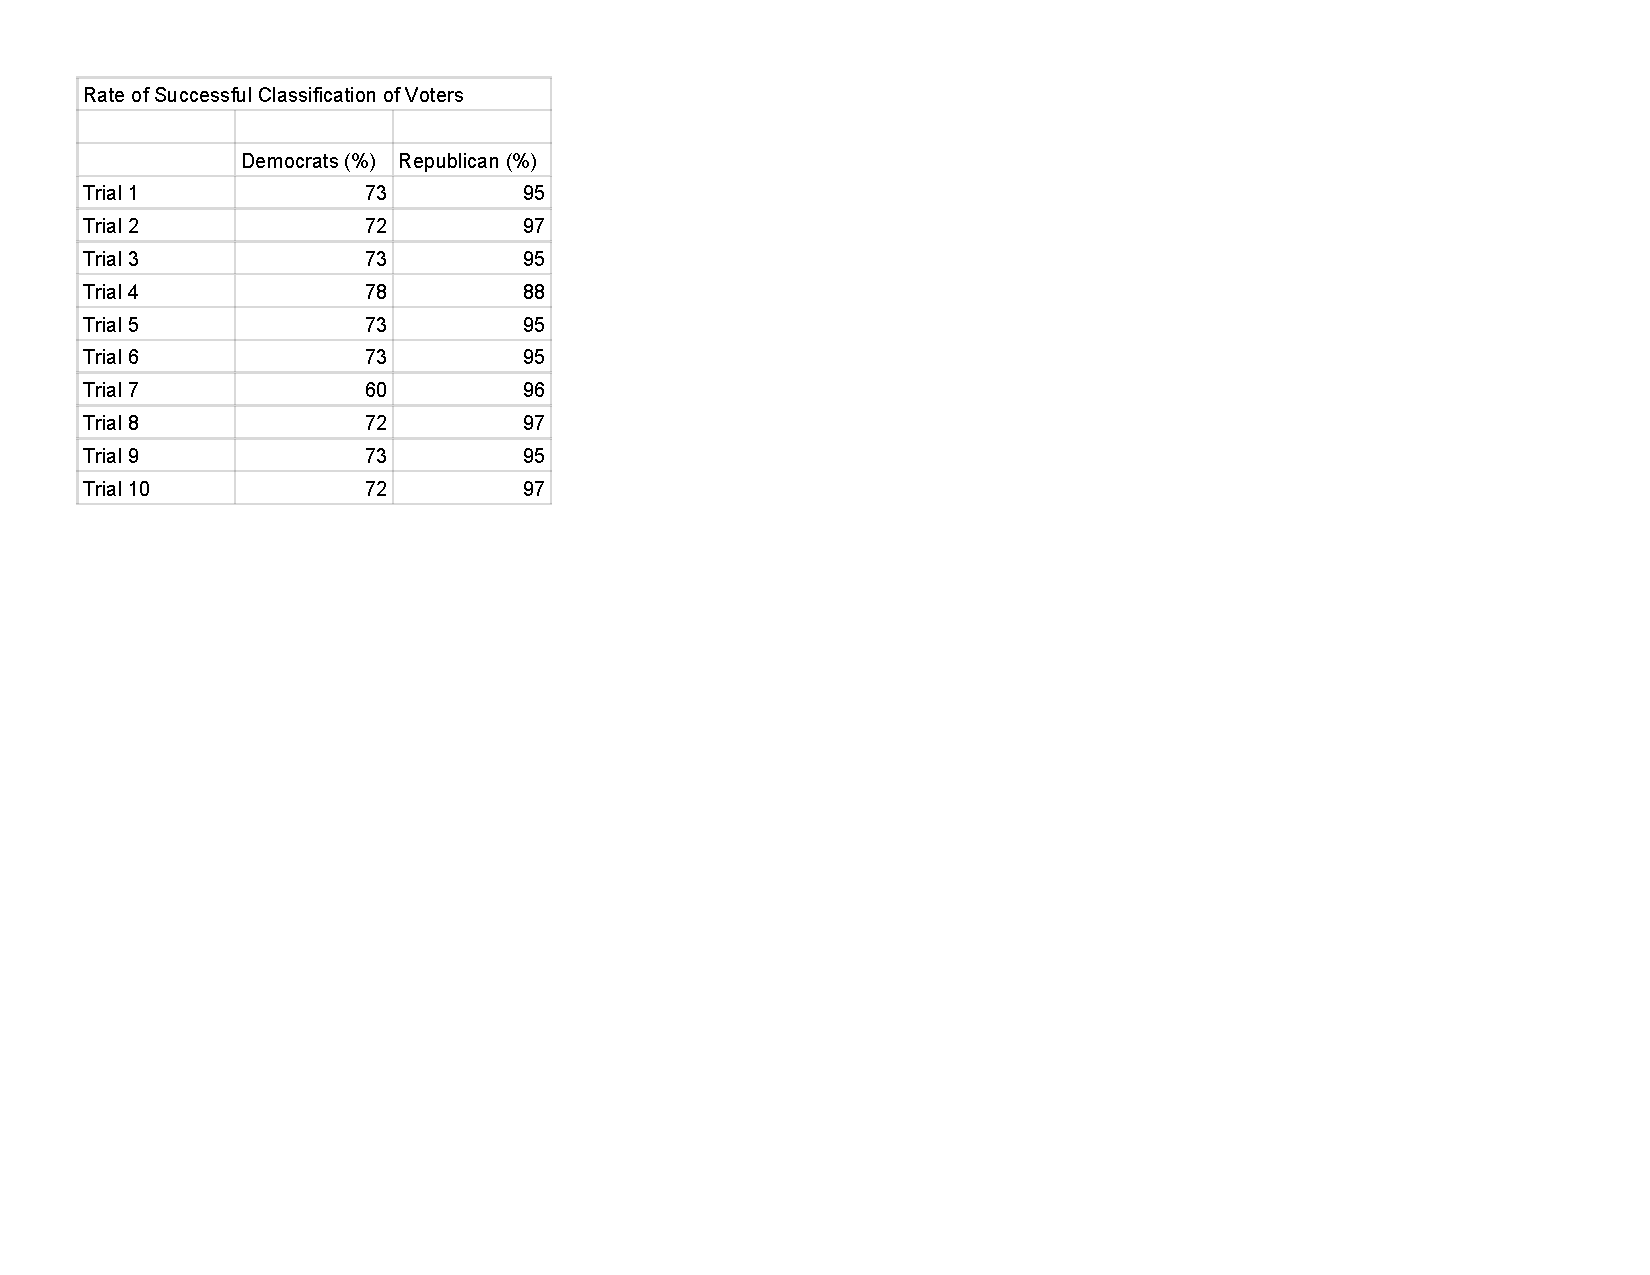
\includegraphics[width=10cm, height=5cm] {voters_classification} 
    }
    \caption{\label{fig:my figure} The rate of correct clustering of democrats and republicans in 10 trials }
    \end{figure}
    
As we can see, the algorithm was reasonably effective, producing over 95\% effective classification for republicans and over 70\% success for democrats in all trials.  Again, we see repeated data, which has me concerned about my algorithm, as I think that with random initialization we should not converge to the same points so much (at least so quickly because I converged after time=3 to 6).  Or I would expect the convergence to yield a higher rate of success in the democrat cluster.  But perhaps these are flaws of the data, and it is not perfect for clustering, I am not sure.  Perhaps a more robust dissimilarity index would help. 



\appendix

\pagebreak

\section*{Appendix 1: K-Means Clustering for Question 1 Matlab Code}
\begin{verbatim}
load('IrisDataAnnotated.mat');

%Intialize k and t and dQ the change in coherence.  will compare t with dQ
k=3;
t=0.00001;
dq=10; old_q=10;
time=1;

%Give random initial partitioning by drawing from array A with #1-150
A=randperm(length([1:150]));
r1=randi([40 60],1); r2=randi([40 60],1);
I_1=A(1:r1);
I_2=A(r1+1:r1+r2);
I_3=A(r1+r2+1:150);

figure
subplot(4,4,time)
scatter3(X(1,I_1),X(2,I_1),X(3,I_1),'r');
hold on
scatter3(X(1,I_2),X(2,I_2),X(3,I_2),'b');
hold on
scatter3(X(1,I_3),X(2,I_3),X(3,I_3),'k');
hold off
title(['K-Means Clustering of Iris Data iteration ' num2str(time)])
xlabel('Sepal length in cm')
ylabel('sepal width in cm')
zlabel('petal length in cm')
pause(1);

dist=zeros(3,150);  

while dq>t
    time=time+1;
    %calculate each cluster's centroid
    c1=sum(X(:,I_1),2)/size(I_1,2);
    c2=sum(X(:,I_2),2)/size(I_2,2);
    c3=sum(X(:,I_3),2)/size(I_3,2);
    
    for ind=1:150
        %calculate distance of each point to each centroid
        dist(:,ind)=[ sqrt(sum((X(:,ind)-c1).^2)) sqrt(sum((X(:,ind)-c2).^2)) sqrt(sum((X(:,ind)-c3).^2))]';
    end
    [m,i]=min(dist);

    
    %assign each data point to cluster with centroid its closest to
    I_1=find(i==1);
    I_2=find(i==2);
    I_3=find(i==3);

    new_q=sum(m);
    dq=abs(new_q-old_q);
    old_q=new_q;

    subplot(4,4,time)
    scatter3(X(1,I_1),X(2,I_1),X(3,I_1),'r');
    hold on
    scatter3(X(1,I_2),X(2,I_2),X(3,I_2),'b');
    hold on
    scatter3(X(1,I_3),X(2,I_3),X(3,I_3),'k');
    hold off
    title(['K-Means Clustering of Iris Data iteration ' num2str(time)])
    xlabel('Sepal length in cm')
    ylabel('sepal width in cm')
    zlabel('petal length in cm')
    pause(1);
end


class=zeros(3,3);
for i=1:size(I_1,2)
    if I(I_1(i))==1
        class(1,1)=class(1,1)+1;
    elseif I(I_1(i))==2
        class(1,2)=class(1,2)+1;
    else
        class(1,3)=class(1,3)+1;
    end
end

for i=1:size(I_2,2)
    if I(I_2(i))==1
        class(2,1)=class(2,1)+1;
    elseif I(I_2(i))==2
        class(2,2)=class(2,2)+1;
    else
        class(2,3)=class(2,3)+1;
    end
end

for i=1:size(I_3,2)
    if I(I_3(i))==1
        class(3,1)=class(3,1)+1;
    elseif I(I_3(i))==2
        class(3,2)=class(3,2)+1;
    else
        class(3,3)=class(3,3)+1;
    end
end


[a,b]=max(class')
setosa=class(find(b==1),:);
versacolor=class(find(b==2),:);
virginica=class(find(b==3),:);




figure(2)
scatter3(X(1,find(I==1)),X(2,find(I==1)),X(3,find(I==1)),'r');
hold on
scatter3(X(1,find(I==2)),X(2,find(I==2)),X(3,find(I==2)),'b');
hold on
scatter3(X(1,find(I==3)),X(2,find(I==3)),X(3,find(I==3)),'k');
hold off
pause(1);

\end{verbatim}
\pagebreak

\section*{Appendix 2: K-Medoids Clustering for Question 1 Matlab Code}
\begin{verbatim}
load('IrisDataAnnotated.mat');

% Intialize k and t and dQ the change in coherence.  will compare t with dQ
k=3;
t=0.00000001;
dq=10; old_q=0;
time=1;
%define a matrix of l1 distance between each point
dist=zeros(150,150);
for i=1:150
    for j=1:150
        dist(i,j)= sum(abs(X(:,i)-X(:,j)));
    end
end

% set 3 random intial medoids
A=randperm(length([1:150]));
m=[X(:,A(1)) X(:,A(2)) X(:,A(3))];
m_ind=[ A(1) A(2) A(3)];

while dq>t
    %Assign each x to nearest medoid
    %find which cluster each x is closest to
    dist_to_all_meds=[dist(:,m_ind(1)) dist(:,m_ind(2)) dist(:,m_ind(3))];
    [dist_to_closest_med, cluster_num]=min(dist_to_all_meds');
    
    %update clusters
    I_1=find(cluster_num==1);
    I_2=find(cluster_num==2);
    I_3=find(cluster_num==3);
    
    figure(1)
    subplot(4,2,time)
    scatter3(X(1,I_1),X(2,I_1),X(3,I_1),'r');
    hold on
    scatter3(X(1,I_2),X(2,I_2),X(3,I_2),'b');
    hold on
    scatter3(X(1,I_3),X(2,I_3),X(3,I_3),'k');
    hold off
    title(['K-Medoids Clustering of Iris Data iteration ' num2str(time)])
    xlabel('Sepal length in cm')
    ylabel('sepal width in cm')
    zlabel('petal length in cm')
    pause(1);
   

    %find best medoid for each cluster
    c1=sum(dist(I_1,I_1));
    [q1,i1]=min(c1);
    m(:,1)=X(:,I_1(i1));
    m_ind(1)=I_1(i1);

    c2=sum(dist(I_2,I_2));
    [q2,i2]=min(c2);
    m(:,2)=X(:,I_2(i2));
    m_ind(2)=I_2(i2);

    c3=sum(dist(I_3,I_3));
    [q3,i3]=min(c3);
    m(:,3)=X(:,I_3(i3));
    m_ind(3)=I_3(i3);
    
    new_q=q1+q2+q3;
    dq=abs(new_q-old_q);
    old_q=new_q;
    time=time+1;
end


class=zeros(3,3);
for i=1:size(I_1,2)
    if I(I_1(i))==1
        class(1,1)=class(1,1)+1;
    elseif I(I_1(i))==2
        class(1,2)=class(1,2)+1;
    else
        class(1,3)=class(1,3)+1;
    end
end

for i=1:size(I_2,2)
    if I(I_2(i))==1
        class(2,1)=class(2,1)+1;
    elseif I(I_2(i))==2
        class(2,2)=class(2,2)+1;
    else
        class(2,3)=class(2,3)+1;
    end
end

for i=1:size(I_3,2)
    if I(I_3(i))==1
        class(3,1)=class(3,1)+1;
    elseif I(I_3(i))==2
        class(3,2)=class(3,2)+1;
    else
        class(3,3)=class(3,3)+1;
    end
end


[a,b]=max(class')
setosa=class(find(b==1),:);
versacolor=class(find(b==2),:);
virginica=class(find(b==3),:);


figure(2)
scatter3(X(1,find(I==1)),X(2,find(I==1)),X(3,find(I==1)),'r');
hold on
scatter3(X(1,find(I==2)),X(2,find(I==2)),X(3,find(I==2)),'b');
hold on
scatter3(X(1,find(I==3)),X(2,find(I==3)),X(3,find(I==3)),'k');
hold off
pause(1);
\end{verbatim}
\pagebreak

\section*{Appendix 3: K-Medoids Clustering for Question 2 Matlab Code}
\begin{verbatim}
load('BiopsyDataAnnotated.mat');
k=2;
t=0.0000001;
dq=10; old_q=0;
time=0;

%define a matrix of euclidean distance between each point
dist=zeros(683,683);
for i=1:683
    for j=1:683
        dist(i,j)= sum(abs(X(:,i)-X(:,j)));
    end
end

% set 3 random intial medoids
A=randperm(length([1:683]));
m=[X(:,A(60)) X(:,A(90))];
m_ind=[A(60) A(90)];


while dq>t
    %Assign each x to nearest medoid
    %find which cluster each x is closest to
    dist_to_all_meds=[dist(:,m_ind(1)) dist(:,m_ind(2))];
    [dist_to_closest_med, cluster_num]=min(dist_to_all_meds');
    
    %update clusters
    I_1=find(cluster_num==1);
    I_2=find(cluster_num==2);

    %find best medoid for each cluster
    c1=sum(dist(I_1,I_1));
    [q1,i1]=min(c1);
    m(:,1)=X(:,I_1(i1));
    m_ind(1)=I_1(i1);

    c2=sum(dist(I_2,I_2));
    [q2,i2]=min(c2);
    m(:,2)=X(:,I_2(i2));
    m_ind(2)=I_2(i2);
    
    new_q=q1+q2;
    dq=abs(new_q-old_q);
    old_q=new_q;
    time=time+1;
end


class=zeros(2,2);  %[benign malignant]
for i=1:size(I_1,2)
    if I(I_1(i))==0
        class(1,1)=class(1,1)+1;
    else
        class(1,2)=class(1,2)+1;
    end
end

for i=1:size(I_2,2)
    if I(I_2(i))==0
        class(2,1)=class(2,1)+1;
    else
        class(2,2)=class(2,2)+1;
    end
end

[a,b]=max(class')
class_benign=class(find(b==1),:);
class_malignant=class(find(b==2),:);

act_malignant=find(I==1); num_malignant=size(act_malignant,2);
act_benign=find(I==0);    num_benign=size(act_benign,2);

sensitivity=class_malignant(2)/num_malignant;
specificity=class_benign(1)/num_benign;
\end{verbatim}
\pagebreak

\section*{Appendix 4: K-Medoids Clustering for Question 3 Matlab Code}
\begin{verbatim}
load('CongressionalVote.mat');

dist=zeros(435,435);
for i=1:435
    for j=1:435
        dissim=0;
        voted=0;
        for k=1:16
            if (X(k,j)~=0) && (X(k,i)~=0);
                voted=voted+1;
                if (X(k,i)~=X(k,j))
                dissim=dissim+1;
                end
            end
        if (voted==0)
            dist(i,j)=1;
        else
            dist(i,j)=dissim/voted;
        end
        end
    end
end
k=2;
t=0.01;
dq=10000; old_q=0;
time=0;


% set 2 random intial medoids
A=randperm(length([1:435]));
m=[X(:,A(20)) X(:,A(50))];
m_ind=[A(20) A(50)];


while dq>t
    %Assign each x to nearest medoid
    %find which cluster each x is closest to

    dist_to_all_meds=[dist(:,m_ind(1)) dist(:,m_ind(2))];
    [dist_to_closest_med, cluster_num]=min(dist_to_all_meds');
    
    %update clusters
    I_1=find(cluster_num==1);
    I_2=find(cluster_num==2);

    %find best medoid for each cluster
    p= dist(I_1,I_1);
    c1=sum(dist(I_1,I_1));
    [q1,i1]=min(c1);
    m(:,1)=X(:,I_1(i1));
    m_ind(1)=I_1(i1);

    c2=sum(dist(I_2,I_2));
    [q2,i2]=min(c2);
    m(:,2)=X(:,I_2(i2));
    m_ind(2)=I_2(i2);
    
    new_q=q1+q2;
    dq=abs(new_q-old_q);
    old_q=new_q;
    time=time+1;
end

act_republicans=find(I==0);    num_republicans=size(act_republicans,2);
act_democrats=find(I==1);     num_democrats=size(act_democrats,2);


class=zeros(2,2);  %[republican democrat]
for i=1:size(I_1,2)
    if I(I_1(i))==0
        class(1,1)=class(1,1)+1;
    else
        class(1,2)=class(1,2)+1;
    end
end

for i=1:size(I_2,2)
    if I(I_2(i))==0
        class(2,1)=class(2,1)+1;
    else
        class(2,2)=class(2,2)+1;
    end
end

[a,b]=max(class')
class_republican=class(find(b==1),:);
class_democrat=class(find(b==2),:);


success_dem=class_democrat(2)/num_democrats;
success_rep=class_republican(1)/num_republicans;
\end{verbatim}

\end{document}


